\section{系统设计与技术路线}
\label{sec:model}
\subsection{总体流程}
拟将系统划分为采集与预处理、统一匿名化、匿名图表情识别和桌面展示四部分。输入先灰度化，再检测人脸并对齐；匿名化模块提供显示画面与标准灰度脸，后者作为表情模型的唯一输入，运行链路与工程职责对应，目录组织拟按图\ref{fig:structure}实施。
\begin{figure}[htbp]
\centering
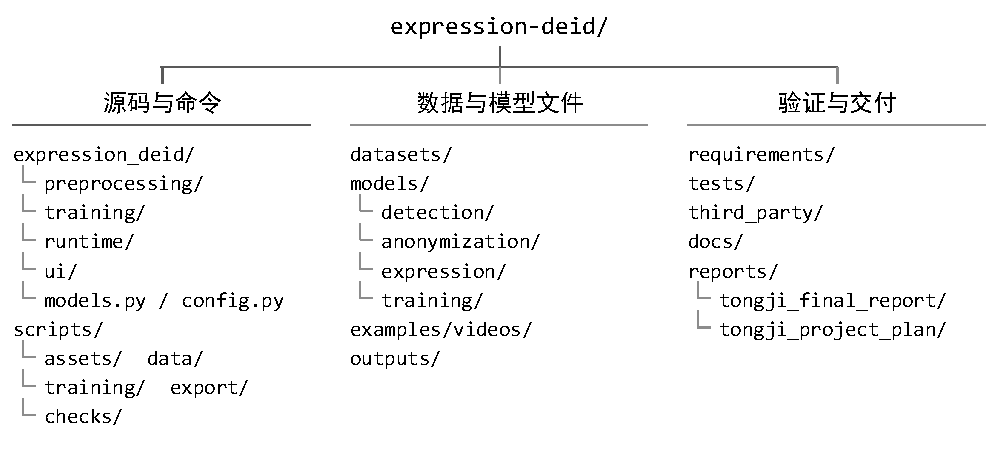
\includegraphics[width=\linewidth]{project_structure.pdf}
\caption{拟采用的工程目录与职责分组}
\label{fig:structure}
\end{figure}

预处理、训练、推理和桌面代码拟分别归入四个子包；训练候选与运行权重分开保存。固定示例输入放入 \path{examples/}，程序生成结果放入 \path{outputs/}，并以同一组检查入口核对各模块的衔接。

\subsection{匿名化模块}
拟使用五点对齐确定面部坐标，在眼眉、鼻部、嘴部及局部纹理区域编辑。软掩膜控制作用范围并合成回灰度画面，面部外区域保留原像素。训练目标兼顾像素变化范围、表情保持、身份抑制与局部平滑，通过项目内身份对照和表情标签共同选择候选。

\subsection{表情识别模块}
拟采用轻量卷积网络作为基线，在通用表情数据上学习后，加入车载近红外样本进行适配。训练分类器之前先生成匿名输入，避免训练只见原图而运行只见匿名图。概率校准和因果时序处理将作为后续优化环节，用于改善置信度的可解释性及视频结果连贯性。

\subsection{桌面端}
计划使用 Python/PySide6 构建原生桌面应用。图片页提供真实标签、原图与匿名图对照及预测结果；视频页支持摄像头、本地视频和示例视频，展示表情、置信度和分析 FPS；表现页汇总数据集结果，便于课堂汇报时从个例过渡到整体评价。

\subsection{GPU 与视频处理}
拟使用 CUDA 加速模型推理，由 PyAV 处理视频编解码，计算任务放入工作线程。优先保证每帧的匿名输入正确，再通过模型预热、实例缓存、检测复用和跟踪减少重复计算。高速与质量配置共用同一接口，分别适应连续演示和准确性优先的分析。
